\documentclass[UTF8,10pt,a4paper,fontset=none]{ctexart}

\usepackage[left=20mm,right=20mm,top=17mm,bottom=18mm]{geometry}
\usepackage{fontspec}
\setmainfont{Liberation Serif}
\setCJKmainfont[BoldFont=Noto Sans CJK SC]{Noto Serif CJK SC}
\setCJKsansfont{Noto Sans CJK SC}
\setCJKmonofont{Noto Sans CJK SC}
\usepackage{amsmath,amssymb,bm}
\usepackage{booktabs,longtable,tabularx,array}
\usepackage{graphicx}
\usepackage{caption,subcaption}
\usepackage{enumitem}
\usepackage{microtype}
\usepackage{titlesec}
\usepackage{multicol}
\usepackage{fancyhdr}
\usepackage{xcolor}
\usepackage{float}
\usepackage{flafter}
\usepackage{placeins}
\usepackage{needspace}
\usepackage[hidelinks]{hyperref}
\usepackage[backend=biber,style=numeric,sorting=none,maxbibnames=4,doi=false,url=false]{biblatex}
\addbibresource{references.bib}
\setlength{\bibitemsep}{0pt}
\setcounter{topnumber}{3}
\setcounter{bottomnumber}{2}
\setcounter{totalnumber}{5}
\renewcommand{\topfraction}{0.92}
\renewcommand{\bottomfraction}{0.85}
\renewcommand{\textfraction}{0.08}
\renewcommand{\floatpagefraction}{0.85}
\setlength{\parindent}{2em}
\setlength{\parskip}{0.08em}
\linespread{1.03}
\setlength{\emergencystretch}{2em}
\setlist{nosep,leftmargin=2.2em}
\renewcommand{\arraystretch}{1.16}
\titleformat{\section}{\bfseries\fontsize{13}{16}\selectfont}{\thesection}{0.65em}{}
\titleformat{\subsection}{\bfseries\fontsize{11.5}{14}\selectfont}{\thesubsection}{0.55em}{}
\titlespacing*{\section}{0pt}{0.85ex plus .2ex}{0.35ex}
\titlespacing*{\subsection}{0pt}{0.55ex plus .2ex}{0.22ex}
\captionsetup{font=normalsize,labelfont=bf,labelsep=quad,justification=justified,singlelinecheck=false}
\renewcommand{\figurename}{图}
\renewcommand{\tablename}{表}
\fancypagestyle{plain}{
  \fancyhf{}
  \fancyhead[L]{\fontsize{8}{10}\selectfont 分子动力学轨迹的生成与检验}
  \fancyhead[R]{\fontsize{8}{10}\selectfont \thepage}
  \renewcommand{\headrulewidth}{0.35pt}
  \renewcommand{\footrulewidth}{0pt}
}
\pagestyle{plain}
\hypersetup{
  pdftitle={从初态到统计结论：分子动力学轨迹的生成与检验},
  pdfauthor={郭铭禹}
}
\begin{document}
\color{black}
\zihao{5}
\raggedbottom
\begin{flushleft}
  {\bfseries\fontsize{17}{21}\selectfont 从初态到统计结论：分子动力学轨迹的生成与检验}\par
  \vspace{5pt}
  {\zihao{5} 郭铭禹}\par
\end{flushleft}
\vspace{2pt}
\hrule
\vspace{6pt}

\begin{abstract}
分子动力学从给定位置、速度和受力出发，通过离散时间推进得到多体轨迹。轨迹的可信度同时取决于三个相互衔接的问题：积分器能否在长时间传播中保留 Hamilton 动力学的几何结构，势能模型能否给出可靠且连续的能量与力，以及有限而相关的轨迹能否支持统计结论。斜抛运动和谐振子分别提供闭式基准与失稳反例，由此可辨认显式 Euler 的相空间膨胀以及 velocity Verlet 的对称、辛和时间可逆结构。势能来源决定每一步的主要成本：经验势把物理假设写入解析函数，AIMD 在每个离子步内迭代电子密度，Deep Potential 以局域环境和原子能分解近似电子结构势能面。系综控制、自相关和增强采样进一步决定轨迹访问哪些状态，以及其中包含多少独立信息。积分误差、势能面误差、系综偏差和统计误差需要分层判断；稳定的能量曲线本身不足以说明轨迹能够支持所报告的物理结论。
\end{abstract}

\noindent\textbf{关键词：} 分子动力学；velocity Verlet；势能面；自洽场；Deep Potential；增强采样

\section{初值问题：位置、速度与受力怎样确定轨迹}

\subsection{斜抛运动中的初态与轨迹}

高中力学里的斜抛运动已经包含了分子动力学的骨架。若忽略空气阻力，初始位置 $\bm r_0$、初始速度 $\bm v_0$ 和恒定重力 $\bm g$ 给定后，任意时刻的位置可直接写成
\begin{equation}
  \bm r(t)=\bm r_0+\bm v_0t+\frac12\bm g t^2.
\end{equation}
这里之所以能“一步到位”，并不是因为牛顿方程天然简单，而是因为加速度恰好为常数。一般的原子体系满足
\begin{equation}
  m_i\ddot{\bm r}_i(t)=\bm F_i(\bm R(t))=-\nabla_i U(\bm R(t)),
  \qquad \bm R=(\bm r_1,\ldots,\bm r_N),
  \label{eq:newton}
\end{equation}
力随所有原子的构型而变，轨迹本身又不断改变下一步的力。问题因而从“代入一个闭式公式”变成了“在时间上反复求解一个耦合初值问题”。

\subsection{两体约化与多体耦合}

“两体问题往往有解析解”需要更谨慎地说。对只依赖两粒子间距的中心力，质心运动可以分离，相对运动可约化成一个等效单粒子问题；但可约化并不等于一定有熟悉的闭式轨道。反平方力和各向同性谐振子是经典可积情形，而一般中心势仍可能需要数值求积。粒子数增加后，方程通常不可积，尽管特殊对称构型、守恒量和特殊解依然存在。分子动力学处理的正是这种常态：不期待写出 $\bm R(t)$ 的闭式表达，而是在有限步长 $\Delta t$ 上构造可信的离散轨迹。

分子动力学的离散推进可写为：
\begin{equation}
  (\bm R_n,\bm V_n)\longrightarrow
  (\bm R_{n+1},\bm V_{n+1}).
\end{equation}
推进公式必须足够稳定，还要尽量保留连续 Hamilton 系统的几何结构。单步看起来很小的偏差，重复几百万次后会变成系统性的漂移。

\section{离散问题：受力怎样推进原子轨迹}

\subsection{显式 Euler 的几何失真}

把式~\eqref{eq:newton}直接按一阶 Taylor 展开，可得到显式 Euler：
\begin{equation}
  \bm R_{n+1}=\bm R_n+\bm V_n\Delta t,
  \qquad
  \bm V_{n+1}=\bm V_n+\bm A(\bm R_n)\Delta t.
  \label{eq:euler}
\end{equation}
位置和速度都只使用旧时刻信息，这一点很关键。若先更新速度，再用新速度更新位置，得到的是辛 Euler；它仍是一阶方法，却具有不同的长期几何性质，不能与式~\eqref{eq:euler}混称。

用频率为 $\omega$ 的一维谐振子 $\ddot q=-\omega^2q$ 可以看清差别。显式 Euler 的更新矩阵为
\begin{equation}
  \begin{pmatrix}q_{n+1}\\v_{n+1}\end{pmatrix}
  =
  \underbrace{\begin{pmatrix}
  1 & \Delta t\\-\omega^2\Delta t & 1
  \end{pmatrix}}_{M_{\mathrm E}}
  \begin{pmatrix}q_n\\v_n\end{pmatrix},
  \qquad
  \det M_{\mathrm E}=1+\omega^2\Delta t^2>1.
\end{equation}
因此每一步都把相平面面积放大。对谐振子而言，数值轨道从本应闭合的椭圆逐渐向外螺旋，能量被系统性注入。缩小步长可以推迟失稳，却没有改变这种误差机制。

能量不守恒为什么是实质问题？微正则系综中的总能量决定可访问的相空间区域。若数值算法持续加热或冷却，轨迹访问的状态、振动频率、扩散行为和时间关联函数都会随之偏移。即便之后加 thermostat 把平均温度拉回目标值，也不代表被扭曲的动力学自动恢复。温控器负责系综采样，积分器负责离散动力学；二者不能互相替罪。

辛 Euler 先做
\begin{equation}
  v_{n+1}=v_n-\omega^2q_n\Delta t,
  \qquad q_{n+1}=q_n+v_{n+1}\Delta t,
\end{equation}
其更新矩阵行列式恰为 $1$。这并不使能量逐步精确不变，却避免了显式 Euler 那种相空间面积的单向膨胀。这个简单例子提示：评价积分器不能只问“单步误差多大”，还要问它长期保留了哪些结构。

\subsection{Hamilton 流的相空间约束}

Hamilton 形式把位置 $\bm q$ 和共轭动量 $\bm p$ 视作相空间坐标：
\begin{equation}
  \dot{\bm q}=\frac{\partial H}{\partial \bm p},
  \qquad
  \dot{\bm p}=-\frac{\partial H}{\partial \bm q},
  \qquad
  H(\bm q,\bm p)=K(\bm p)+U(\bm q).
\end{equation}
Liouville 定理说明精确 Hamilton 流保持相空间体积。辛性则是更强的几何条件：时间推进映射保持辛二形式，因此不仅保体积，也保留 Hamilton 动力学中位置与动量的配对结构。对常见的可分 Hamiltonian，Verlet 家族可以看成动能流和势能流的对称分裂；每个子流都可精确求解，组合后仍是辛映射\cite{hairer2006}。

四个常被混用的概念需要分开：
\begin{itemize}
  \item \textbf{相空间体积保持}只要求 Jacobian 行列式为一；它弱于辛性。
  \item \textbf{辛性}约束离散映射的几何结构，但不保证每一步精确保持原 Hamiltonian。
  \item \textbf{时间可逆性}要求用 $-\Delta t$ 能沿同一离散路径返回；对平衡态动力学尤其有价值。
  \item \textbf{能量守恒}若指 $H_n=H_0$ 逐步精确成立，常规 velocity Verlet 并不满足。
\end{itemize}
Velocity Verlet 的长期优势来自后向误差分析：在足够小的步长下，离散轨迹可以理解为某个邻近的 shadow Hamiltonian 的精确轨迹，因此原 Hamiltonian 的误差通常围绕零作有界振荡，而不是像显式 Euler 那样单向漂移\cite{hairer2006}. “能量表现好”是这种结构的结果，不应被简化成“Verlet 精确守恒能量”。

\subsection{Velocity Verlet 的对称离散}

位置 Verlet 可由正、反向 Taylor 展开相加得到：
\begin{equation}
  \bm R_{n+1}=2\bm R_n-\bm R_{n-1}+\bm A_n\Delta t^2+\mathcal O(\Delta t^4).
\end{equation}
它只显式推进位置，速度需要另行估计。Leapfrog 把速度放在半步：
\begin{align}
  \bm V_{n+1/2}&=\bm V_{n-1/2}+\bm A_n\Delta t,\\
  \bm R_{n+1}&=\bm R_n+\bm V_{n+1/2}\Delta t.
\end{align}
Velocity Verlet 则让整步位置和速度同时可用\cite{swope1982}：
\begin{align}
  \bm R_{n+1}&=\bm R_n+\bm V_n\Delta t+\frac12\bm A_n\Delta t^2,
  \label{eq:vv-r}\\
  \bm A_{n+1}&=\bm M^{-1}\bm F(\bm R_{n+1}),
  \label{eq:vv-a}\\
  \bm V_{n+1}&=\bm V_n+\frac12(\bm A_n+\bm A_{n+1})\Delta t.
  \label{eq:vv-v}
\end{align}
真正昂贵的通常是式~\eqref{eq:vv-a}：新位置确定后必须重新评价势能及其梯度。式~\eqref{eq:vv-r}--\eqref{eq:vv-v}因此也自然形成“位置--加速度--速度”的三节点循环。若下一步继续推进，$\bm A_{n+1}$ 可直接复用，每个时间步只需一次新的力计算。

固定步长 classical RK4 对一般常微分方程具有四阶全局精度，短时间误差显著小于二阶 Verlet；但标准 RK4 不是辛方法，每步还要多次评价右端项。分子动力学中一次力计算可能意味着一轮昂贵电子结构计算，此时“用四倍力计算换更高阶”未必划算。更重要的是，高阶局部精度不自动转化成长时间统计性质。RK4 很适合短时间高精度传播、非 Hamilton 系统或作为参考解；对长时间、近保守的原子动力学，velocity Verlet 往往以较低成本提供更合适的误差结构。

\begin{table}[htbp]
\centering
\caption{常见固定步长积分器的性质。这里“力/步”按无额外复用的一般实现计；具体程序可复用端点力。}
\small
\begin{tabularx}{\textwidth}{lcccccX}
\toprule
方法 & 全局阶 & 辛 & 可逆 & 力/步 & 长期能量 & 典型用途 \\
\midrule
显式 Euler & 1 & 否 & 否 & 1 & 常系统漂移 & 教学反例、极短步调试 \\
辛 Euler & 1 & 是 & 否 & 1 & 有界但偏差较大 & 几何积分入门 \\
Leapfrog & 2 & 是 & 是 & 1 & 有界振荡 & 经典 MD \\
Velocity Verlet & 2 & 是 & 是 & 1 & 有界振荡 & 经典 MD、AIMD、MLIP-MD \\
RK2 & 2 & 通常否 & 通常否 & 2 & 可出现长期漂移 & 一般 ODE \\
Classical RK4 & 4 & 否 & 否 & 4 & 短时很准，长期可漂移 & 参考传播、非保守问题 \\
\bottomrule
\end{tabularx}
\end{table}

\begin{figure}[htbp]
  \centering
  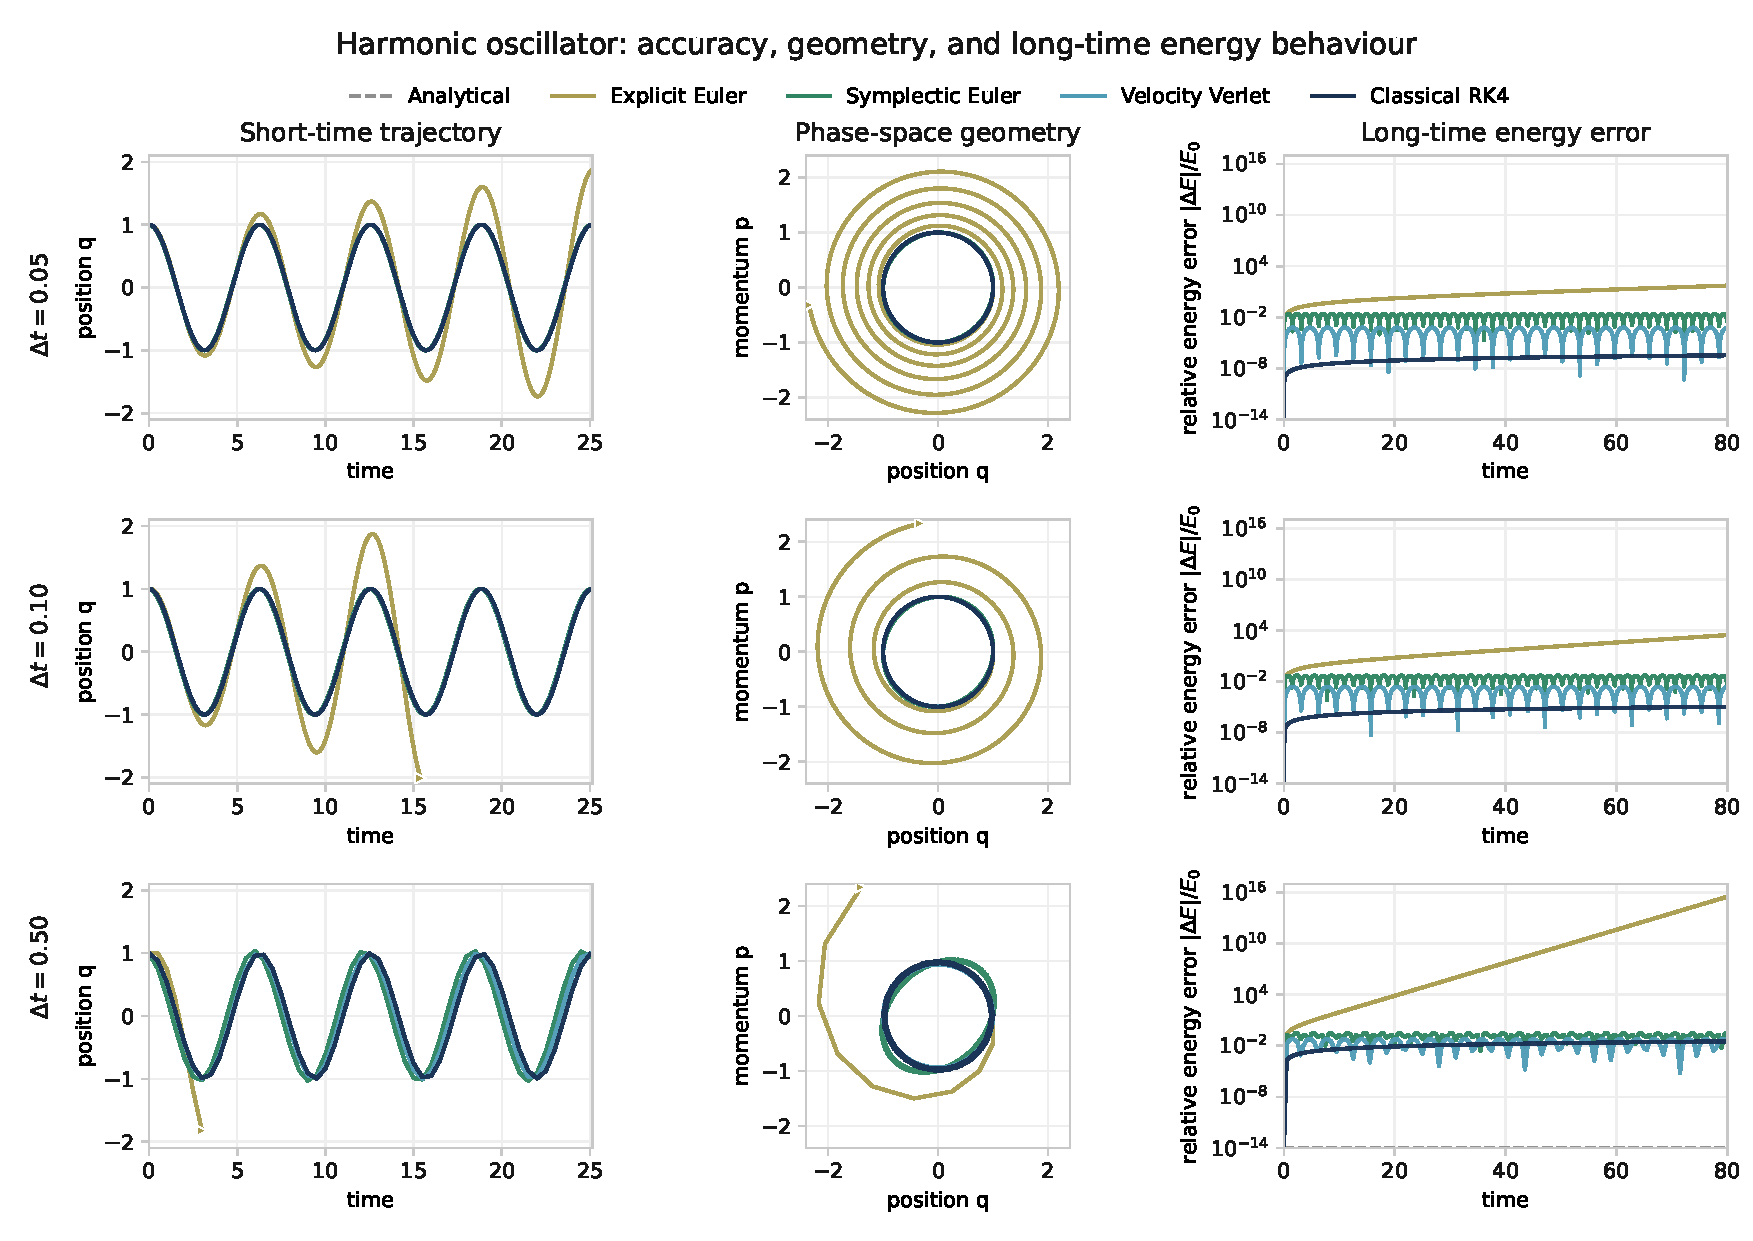
\includegraphics[width=0.96\textwidth]{../integrator_animations/figures/integrator_comparison.pdf}
  \caption{谐振子上对积分器的统一比较：短时轨迹、相空间几何和长期相对能量误差。配套 Notebook 的步长收敛测试给出 velocity Verlet 的实测阶数 2.004 和 2.001，与二阶全局误差一致。}
  \label{fig:integrators}
\end{figure}

步长仍需由体系的最快自由度决定。含氢体系的高频伸缩常迫使 $\Delta t$ 落在飞秒量级；若对键长施加 SHAKE/RATTLE 约束，可以移除最快振动并使用更大步长，但约束算法本身也必须与积分器和温控器一致。判断步长不能只看一次轨迹“没有炸”，至少要比较能量漂移、结构分布、时间关联函数和目标观测量的步长收敛。

\section{势能问题：原子构型怎样给出力}

所有上述积分器都把力当作可调用的函数。原子构型到加速度的映射可写为
\begin{equation}
  \bm R_n\longrightarrow U(\bm R_n)
  \longrightarrow \bm F_n=-\nabla_{\bm R}U(\bm R_n)
  \longrightarrow \bm A_n
  \longrightarrow \text{integrator}.
  \label{eq:pes-loop}
\end{equation}
积分器回答“如何从当前状态走到下一步”，势能面回答“地形是什么、坡朝哪里”。同一积分器配上不同势函数，会得到完全不同的物理；反过来，再准确的势能面若搭配失稳的推进方法，也无法产生可信的长时间轨迹。

势能 $U(\bm R)$ 是 $3N$ 维构型空间上的标量函数。图上常画的一维曲线只是某条反应坐标切片。真正的力是高维梯度，每个原子都有三个分量。这里还隐含一个一致性要求：若模型先预测总能量，再通过自动微分取负梯度，力天然是保守的；若能量和力由彼此独立的输出头直接拟合，则需要额外检查两者是否可积以及长期 NVE 能量表现。

\subsection{经验势的解析相互作用}

经验势把电子自由度积分掉，用预先选定的函数形式近似原子间相互作用。Lennard--Jones 势
\begin{equation}
  U_{\mathrm{LJ}}(r)=4\epsilon\left[\left(\frac{\sigma}{r}\right)^{12}
  -\left(\frac{\sigma}{r}\right)^6\right]
\end{equation}
以短程排斥和色散吸引构成最简单的范例\cite{jones1924}. 其径向力为
\begin{equation}
  F_r(r)=-\frac{\mathrm d U}{\mathrm d r}
  =24\epsilon\left[2\frac{\sigma^{12}}{r^{13}}-
  \frac{\sigma^6}{r^7}\right].
\end{equation}
实现时应以有限差分核对解析导数，并检查截断处是否需要平移、切换函数或长程修正。一个符号错误就会把吸引变成排斥，而这种错误在复杂动画中反而可能被视觉效果掩盖。

水模型说明了“一个 LJ 项”与“完整力场”的区别。TIP3P 等固定电荷模型通常在氧--氧之间使用 LJ 项，同时包含原子部分电荷间的静电作用，并以键长、键角约束或势项维持分子内几何\cite{jorgensen1983}. 因此在水二聚体上突出 $r_{\mathrm{OO}}\to U_{\mathrm{LJ}}\to F\to a$ 是一种局部解释，不应暗示氢键完全由 LJ 描述。经验势速度快，是因为函数形式和参数已经把大量电子结构响应压缩掉；它的局限也来自同一处：电荷转移、成键断键、极化和跨化学空间外推通常需要额外模型或重新参数化。

Fermi--Pasta--Ulam 1955 年的数值实验研究非线性振子链的能量弛豫，是计算动力学史上的标志性工作，但把它称作第一项标准分子动力学模拟并不严谨\cite{fpu1955}. Alder 与 Wainwright 1957 年对硬球体系的研究通常被列为早期经典 MD 里程碑\cite{alder1957}；Rahman 1964 年用 Lennard--Jones 势模拟液氩，展示了从原子轨迹计算液体结构和动力学关联的路径\cite{rahman1964}；Verlet 1967 年重新组织并推广了后来广泛使用的位置递推形式\cite{verlet1967}. 沿着这条历史线，轨迹、统计力学和可计算势函数逐渐闭合成一套实践方法。

\begin{figure}[htbp]
  \centering
  \begin{subfigure}[t]{0.485\textwidth}
    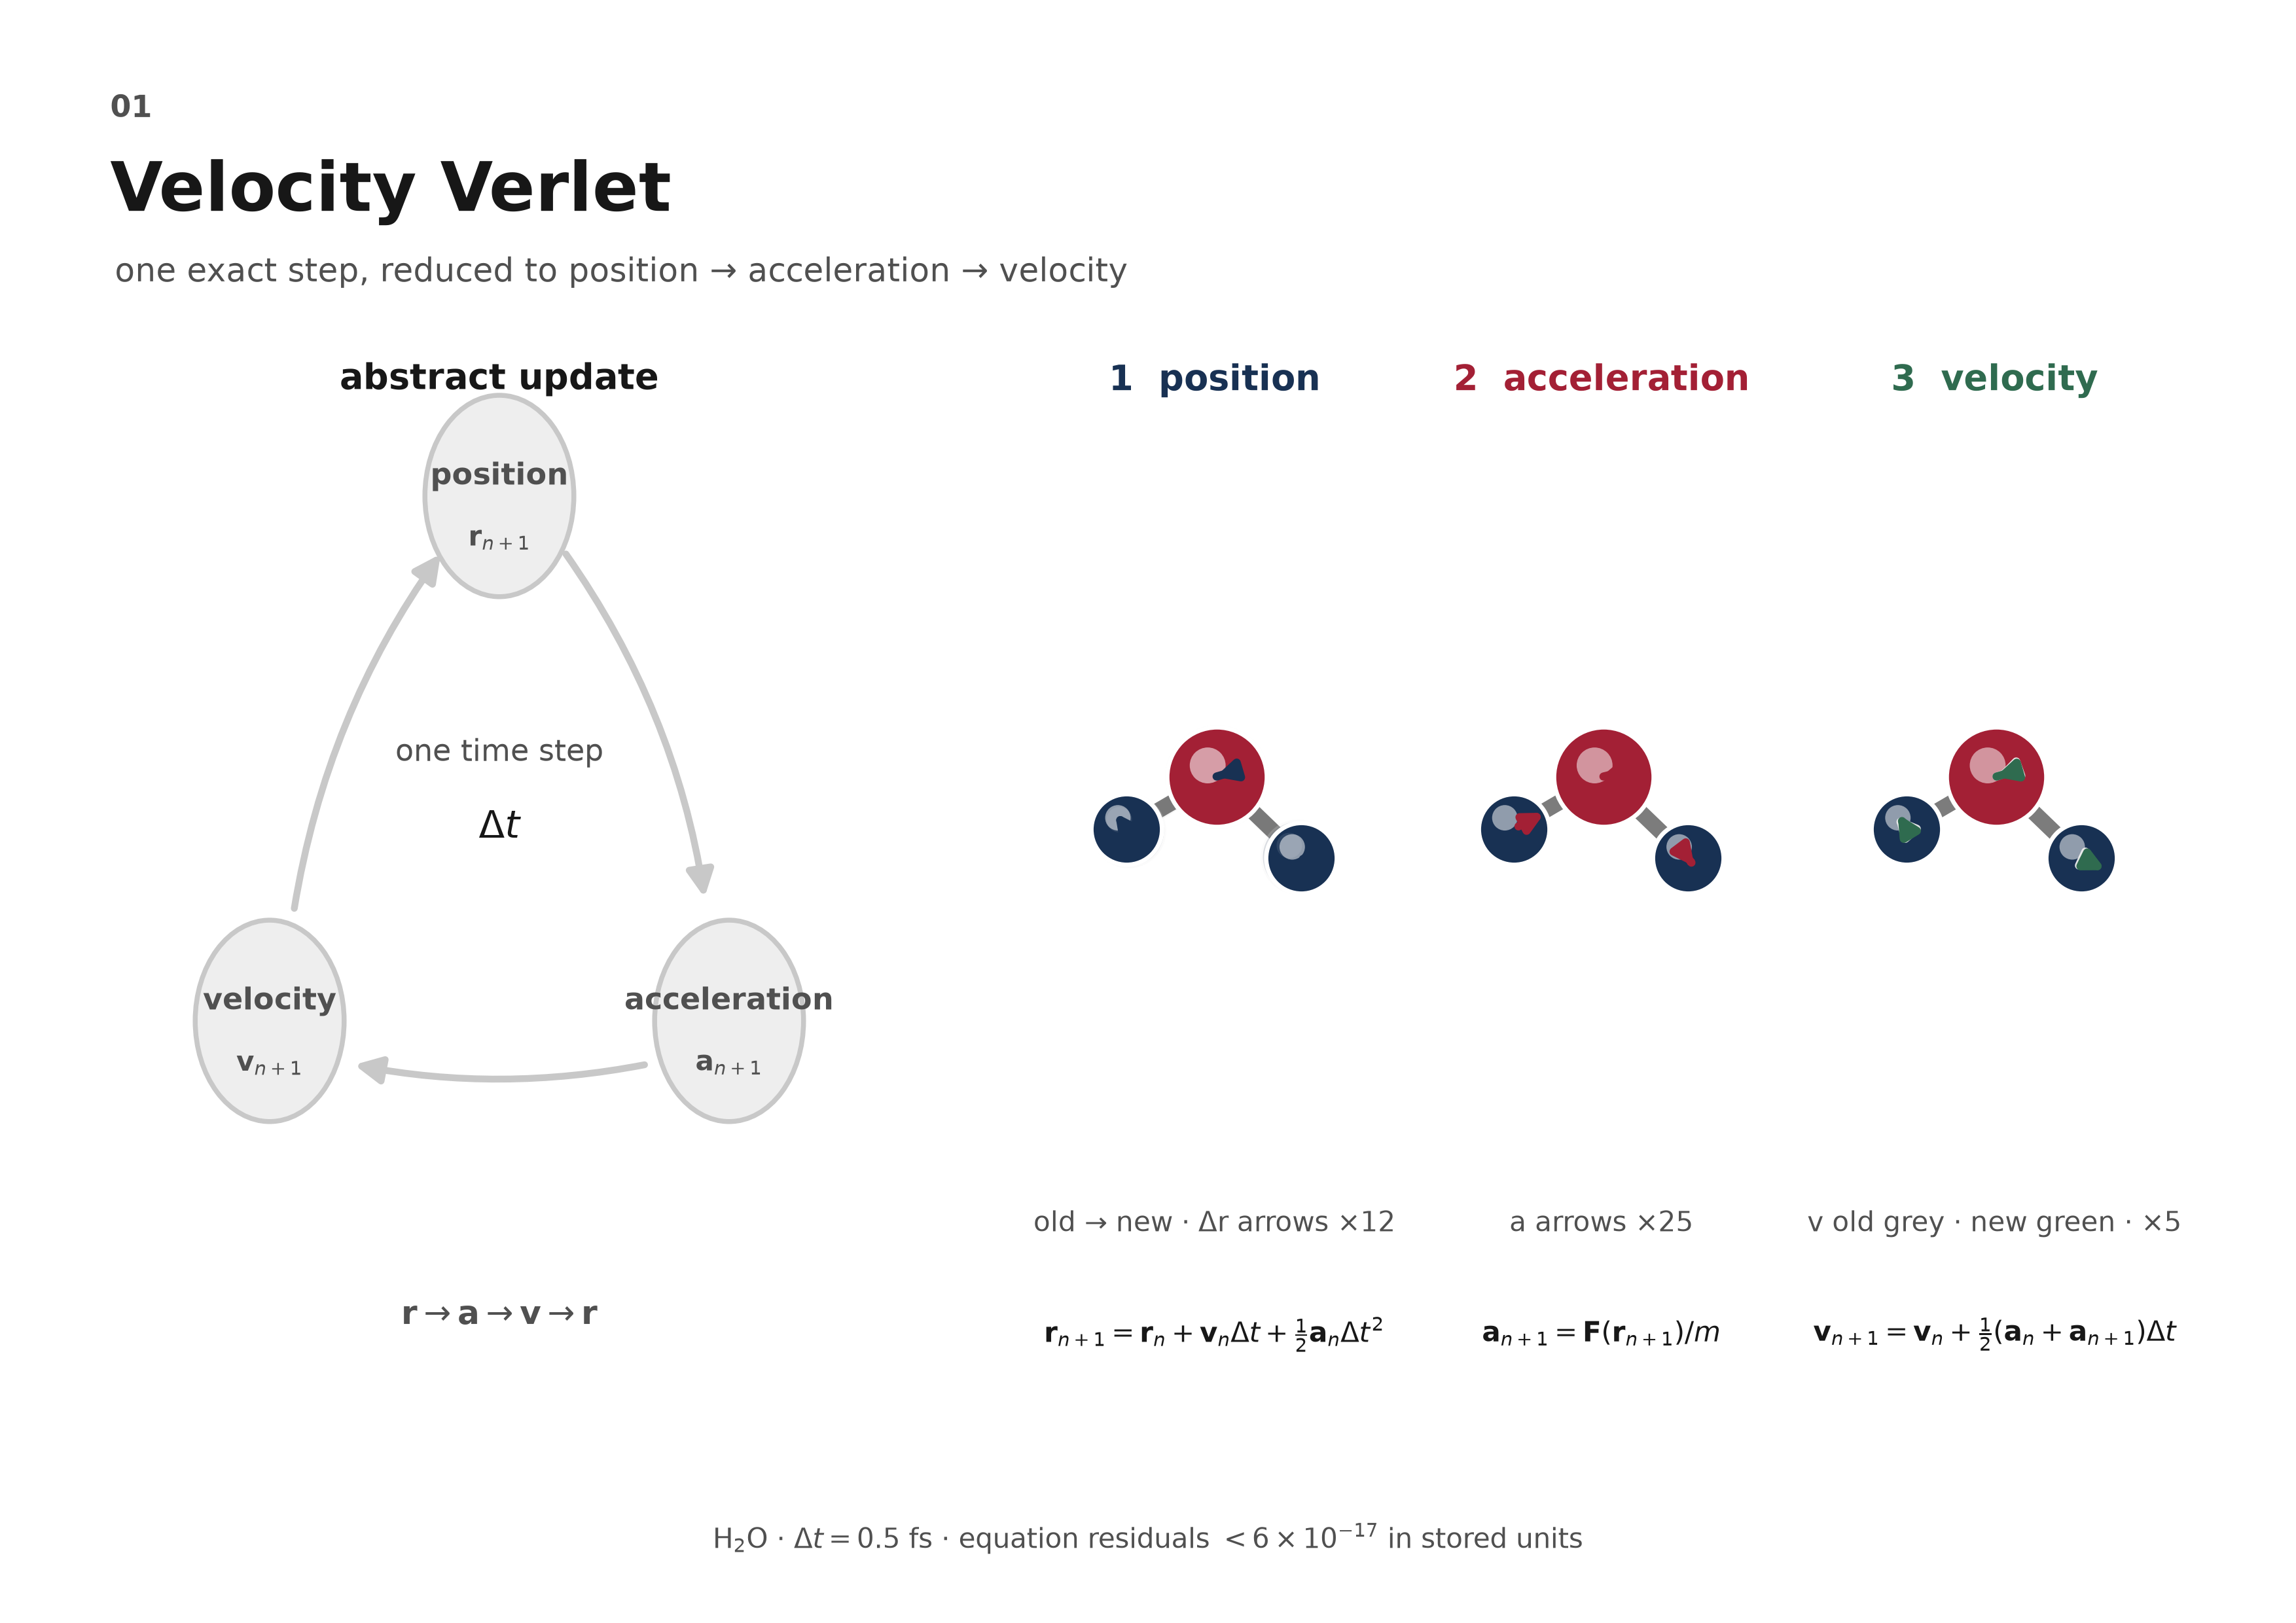
\includegraphics[width=\linewidth]{../four_part_story/figures/01_velocity_verlet.png}
    \caption{Velocity Verlet：抽象三步与真实水分子运动。}
  \end{subfigure}\hfill
  \begin{subfigure}[t]{0.485\textwidth}
    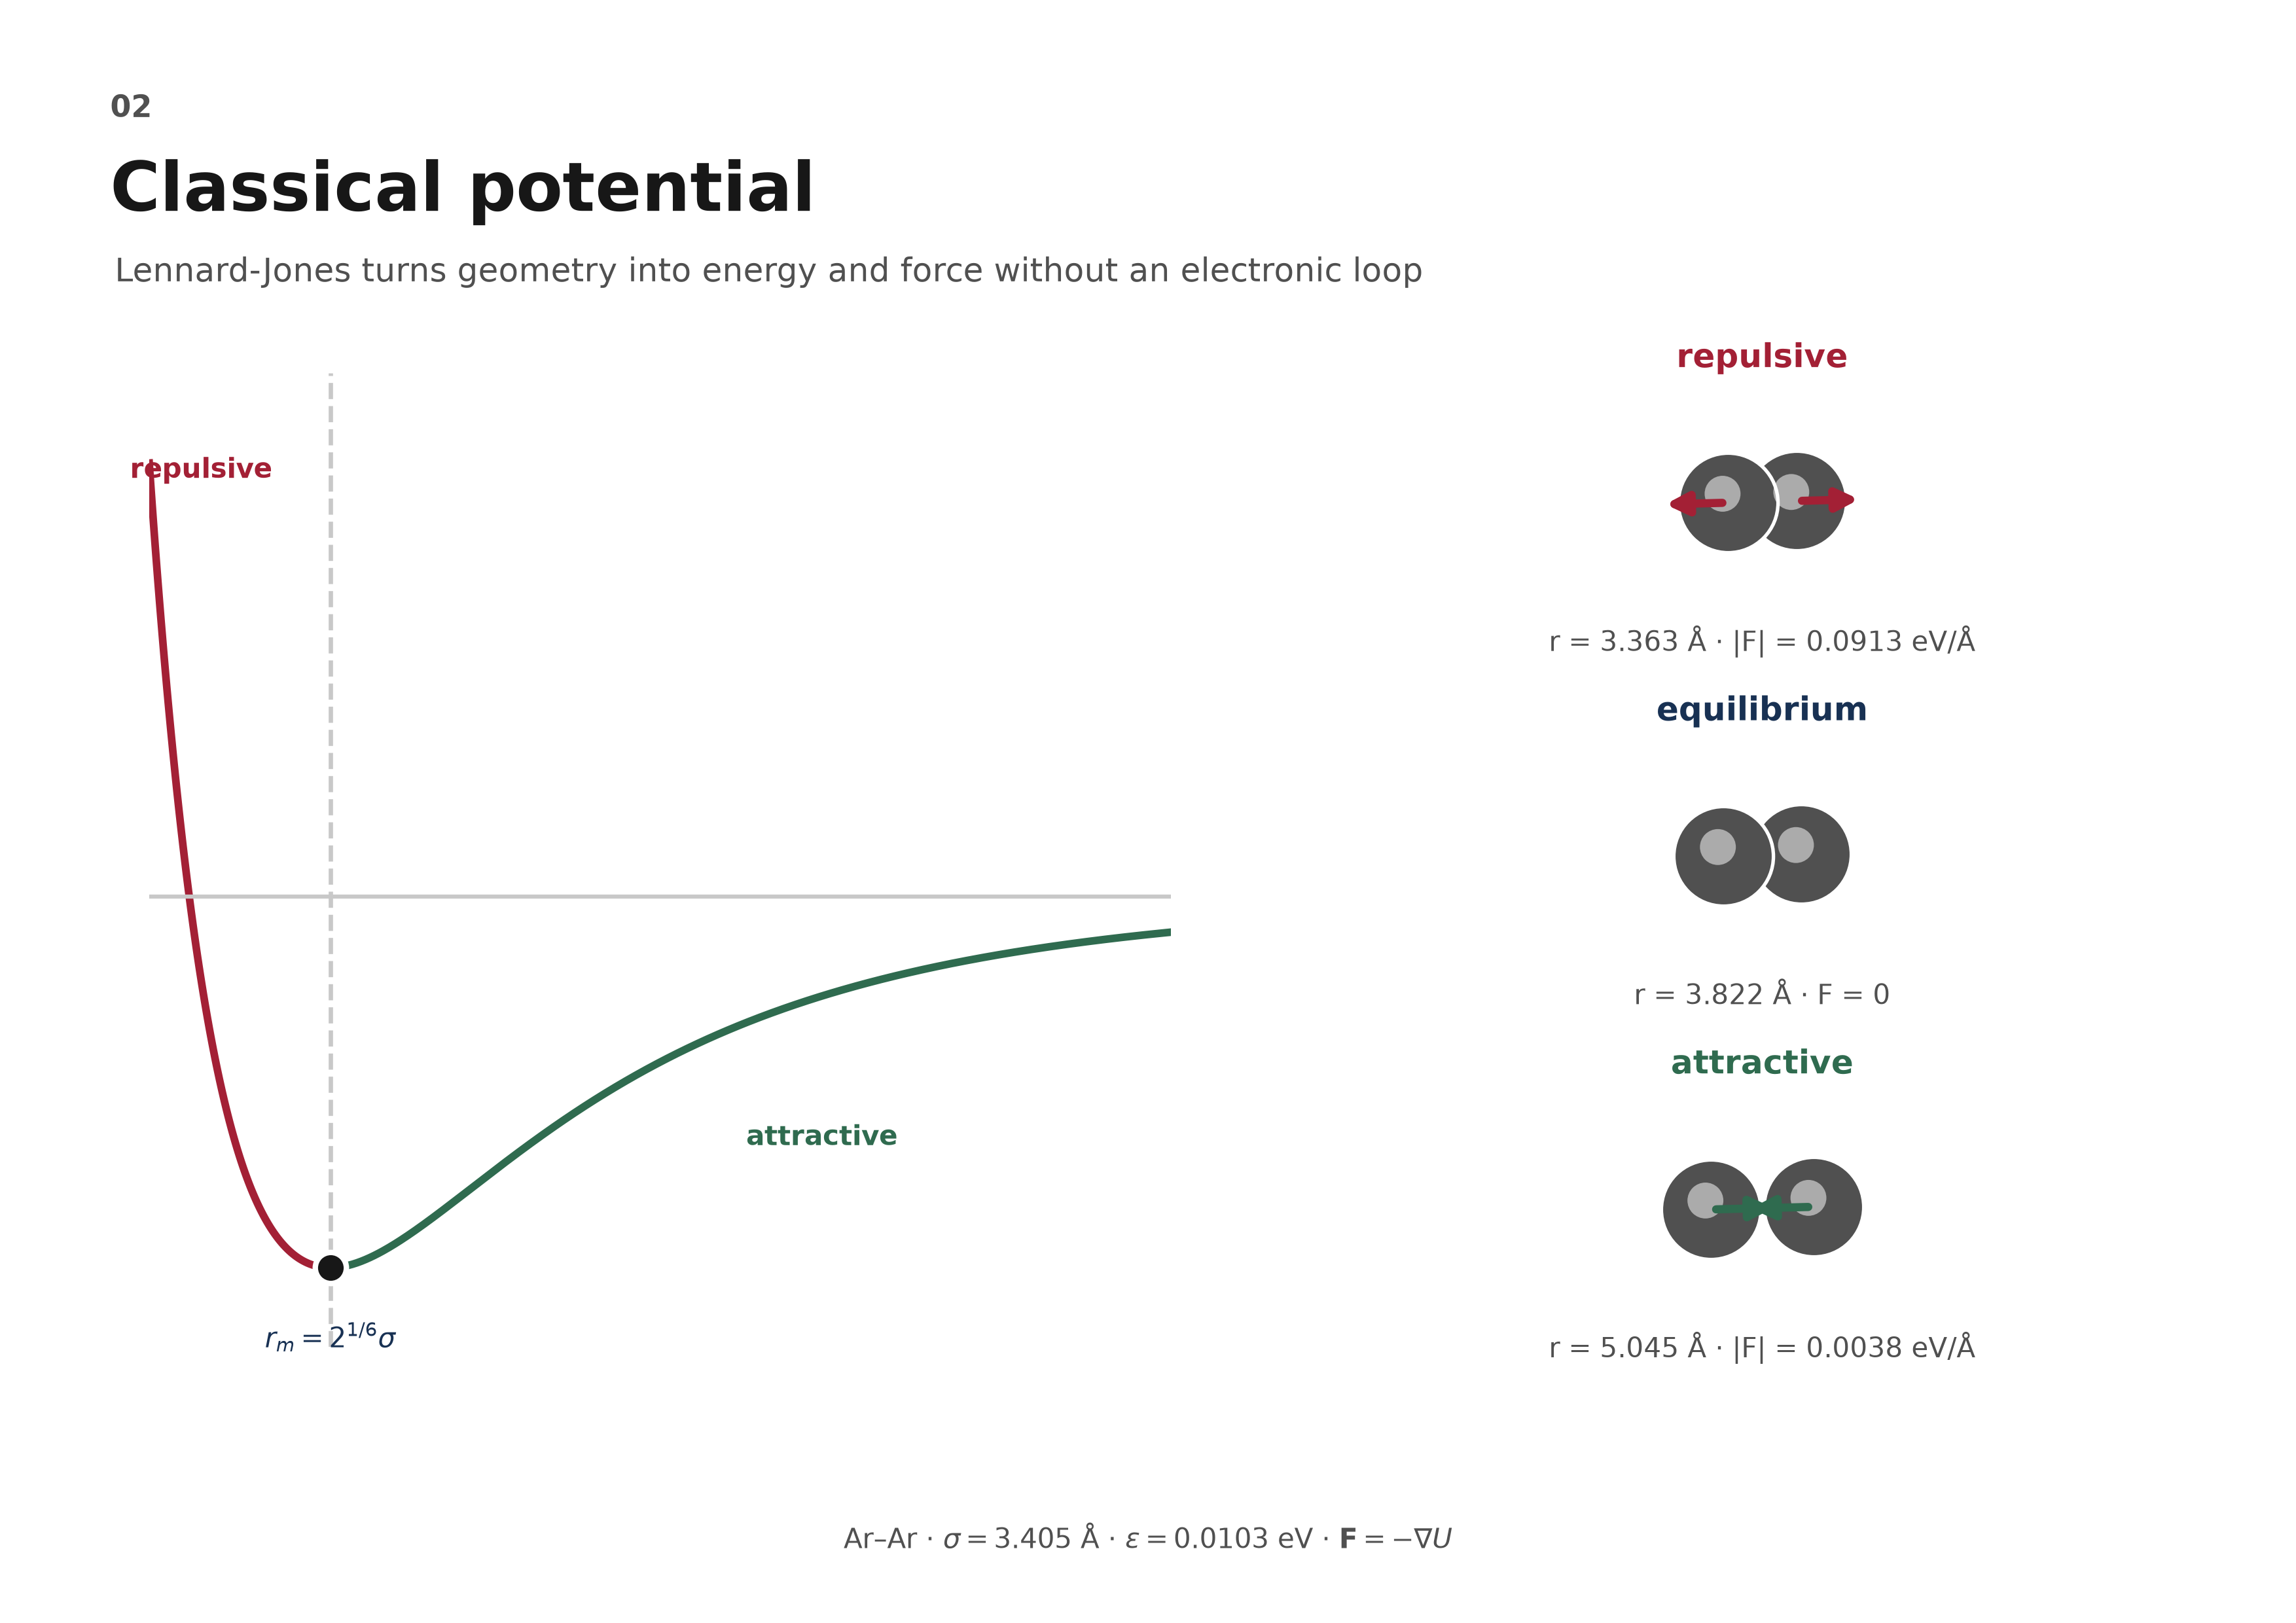
\includegraphics[width=\linewidth]{../four_part_story/figures/02_classical_lj.png}
    \caption{经典势：水二聚体上的 O--O LJ 力。}
  \end{subfigure}
  \caption{Velocity Verlet 与经验势在水体系中的具体对应。左图显示位置、加速度和速度的离散更新及单个水分子的位移；右图以水二聚体的 O--O 距离说明解析势能、力与加速度之间的关系。}
  \label{fig:vv-lj}
\end{figure}

\subsection{AIMD 的电子自洽力}

从头算分子动力学不预先拟合固定解析势，而是在每个离子构型上求电子基态能量，再由 Hellmann--Feynman 力及必要的 Pulay 修正推进原子。Born--Oppenheimer 近似利用电子与原子核质量尺度差异，把核在一张电子基态势能面上的运动与电子问题分开\cite{born1927}. 对 Hartree--Fock 或 Kohn--Sham DFT，电子方程又是非线性的：轨道决定密度，密度决定有效势或 Fock 矩阵，而它们反过来决定新轨道。

一个自洽场循环可以写成
\begin{equation}
  P^{(k)} \xrightarrow{\text{构造 Fock}}
  F[P^{(k)}] \xrightarrow{\text{解本征问题}}
  C^{(k+1)} \xrightarrow{\text{占据}}
  P_{\mathrm{out}}^{(k+1)}
  \xrightarrow{\text{混合}} P^{(k+1)}.
\end{equation}
迭代直到能量差、密度矩阵残差或交换子残差满足阈值。Roothaan 方程奠定了基组中的闭壳层 Hartree--Fock 自洽形式\cite{roothaan1951}；DIIS 等外推方法通过残差子空间加速并稳定收敛\cite{pulay1980}. 重要的是，SCF 总能量并不保证每次迭代单调下降；混合、阻尼和 DIIS 可能造成局部回升，但只要残差最终收敛，不能据此判定计算错误。

计算量大的来源由此变得直观：一次离子步不是一次矩阵求解，而是多次“构造--求解--更新--判断”的电子步；每个电子步又包含随基组规模增长的线性代数和双电子项处理。若前一步收敛密度被用作下一离子步初猜，通常可显著减少迭代次数；但体系发生电荷重排、能级交叉或几何突变时，SCF 仍可能变慢或失败。20 世纪 90 年代围绕密度矩阵局域性、稀疏表示和避免全局对角化的研究，目标正是把绝缘体电子结构从传统立方标度推向近线性标度\cite{goedecker1999}。

Born--Oppenheimer MD 在每个离子步把电子自由度收敛到基态，再计算核力。Car--Parrinello MD 则引入电子轨道的虚拟质量，把轨道和离子放在扩展 Lagrangian 中联合传播\cite{carparrinello1985}. Car--Parrinello MD 的算法逻辑不同；它用绝热分离和受约束电子动力学保持轨道接近瞬时基态。虚拟质量、时间步和电子--离子能量交换必须仔细控制。现代实现中，BOMD 配合高效 SCF、外推和预条件往往更直接；CPMD 仍有重要历史和方法学价值。

二维密度等值图比三维等值面更适合水二聚体的教学动画：分子平面、网格、色标和等值线水平固定后，可以把 $\rho^{(k)}(\bm r)$ 的真实变化与 SCF 残差控制的视觉平滑结合起来。初猜阶段轮廓宽而粗糙，迭代推进时逐渐清晰；相邻迭代必须插值，且禁止逐帧自动缩放，否则观众看到的只是闪烁而不是收敛。收敛后停顿，再分阶段显示核梯度、速度更新和位置漂移，才把“电子步嵌套在离子步内”的层级说清楚。

\begin{figure}[htbp]
  \centering
  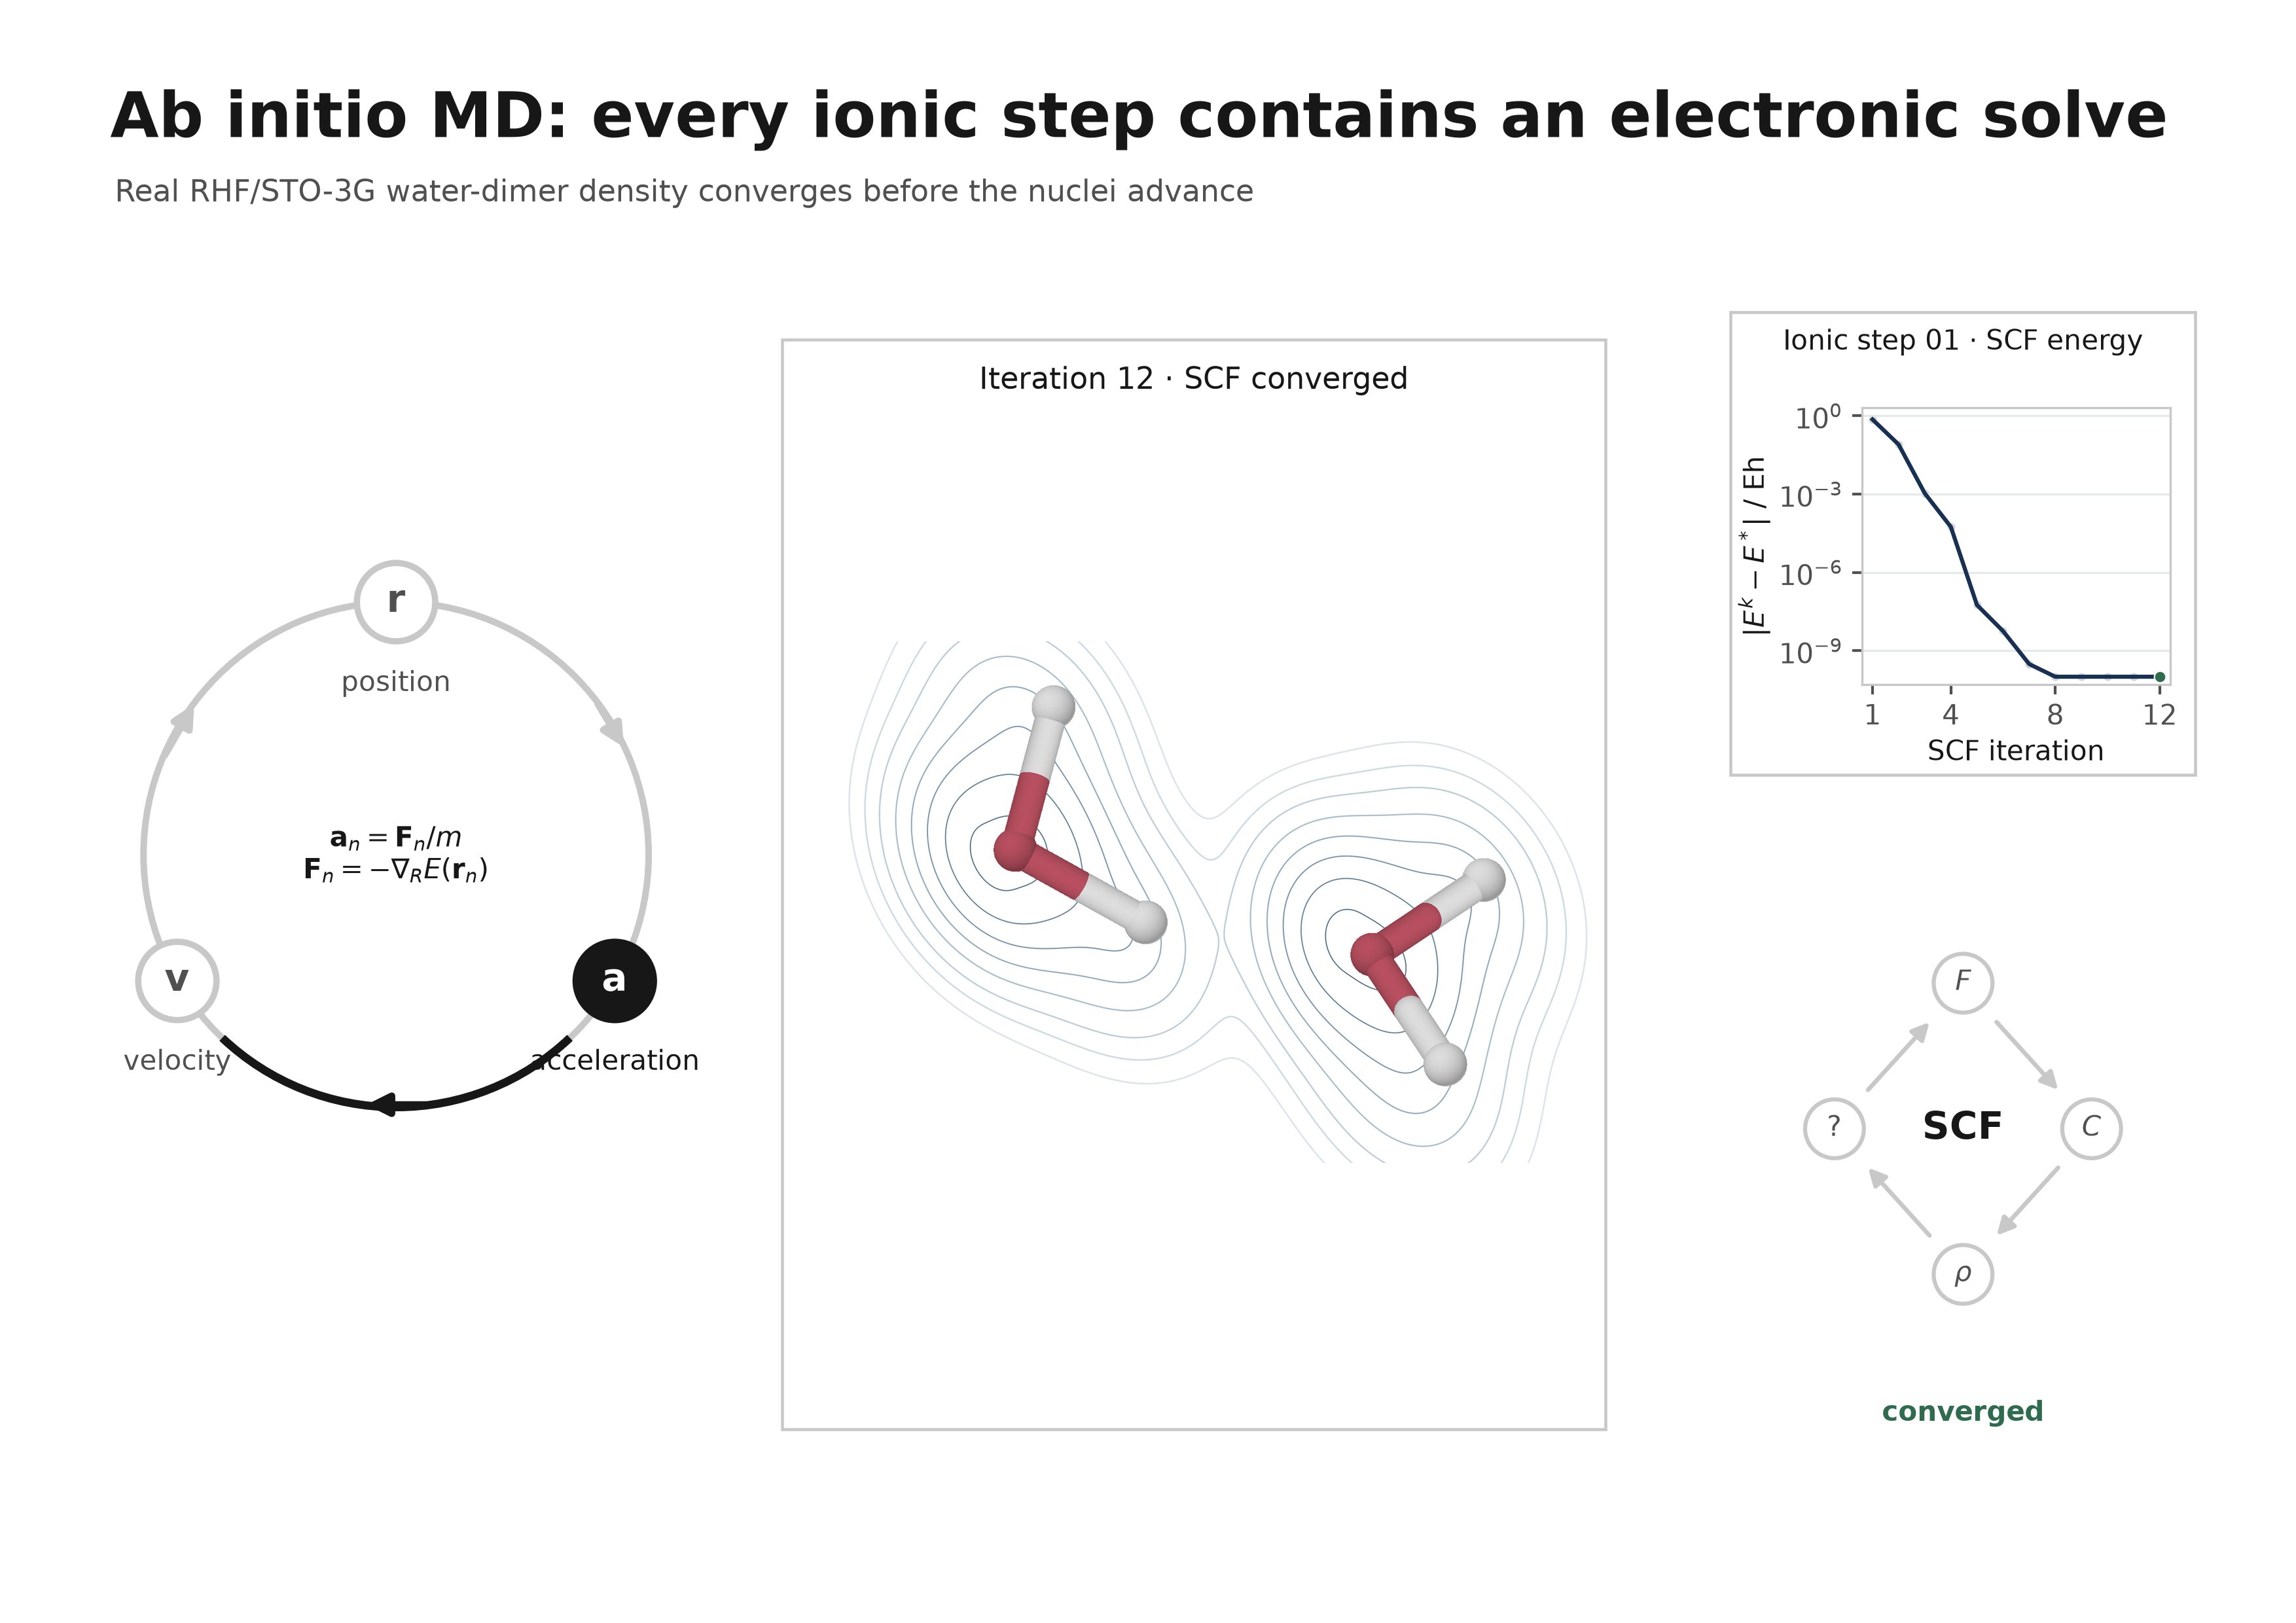
\includegraphics[width=0.93\textwidth]{../four_part_story/figures/03_aimd_scf.png}
  \caption{AIMD 中电子步与离子步的嵌套关系。每个离子构型先经过 SCF 迭代得到收敛电子密度和核力，随后更新速度与位置并进入下一离子步。}
  \label{fig:aimd}
\end{figure}

\subsection{Deep Potential 的局域能量分解}

经验势把先验写进有限的解析形式；机器学习原子间势（MLIP）则从电子结构标注的能量、力和应力中学习更灵活的函数。Behler--Parrinello 高维神经网络势把总能量写成原子能之和，并用对平移、旋转和同种原子置换不变的局域描述符表示环境\cite{behler2007}. GAP 随后以高斯过程和 SOAP 等核表示给出带不确定性和系统可改进性的路线\cite{bartok2010}. 两者共同确立了一个关键范式：高维势能面可以通过局域环境分解来学习，而不是直接把整个 $3N$ 维坐标向量塞进一个黑箱。

Deep Potential 的里程碑意义在于把对称性保持的局域表示、端到端能量模型、自动微分力和大规模并行 MD 结合成完整体系\cite{han2018,zhang2018deepmd}. 对中心原子 $i$，在截断半径 $r_c$ 内收集邻居 $j$，由相对向量 $\bm r_{ij}$ 构造平滑环境表示，再通过共享网络得到原子能 $E_i$：
\begin{equation}
  E(\bm R)=\sum_i E_i(\mathcal N_i),
  \qquad
  \bm F_i=-\frac{\partial E}{\partial \bm r_i}.
  \label{eq:dp}
\end{equation}
平移不变性来自相对坐标；旋转和置换对称性由描述符或等变网络结构编码；局域截断使计算量随原子数近线性增长。这里的“近线性”指固定密度、固定截断和有效邻居表下的推理复杂度，不意味着训练数据生成也便宜，更不意味着长程静电和非局域电子效应会自动消失。

Deep Potential 的局域计算可由同一快照中的数据链展开：中心原子周围 $6$~\AA{} 截断球内的周期最小镜像邻居构成局域环境，环境表示经过共享网络得到原子能，各原子能相加形成总能量并由其梯度给出力。中心原子、邻居列表、原子能、总能量和力必须来自同一次计算，才能保持这一映射的物理一致性。

\begin{figure}[htbp]
  \centering
  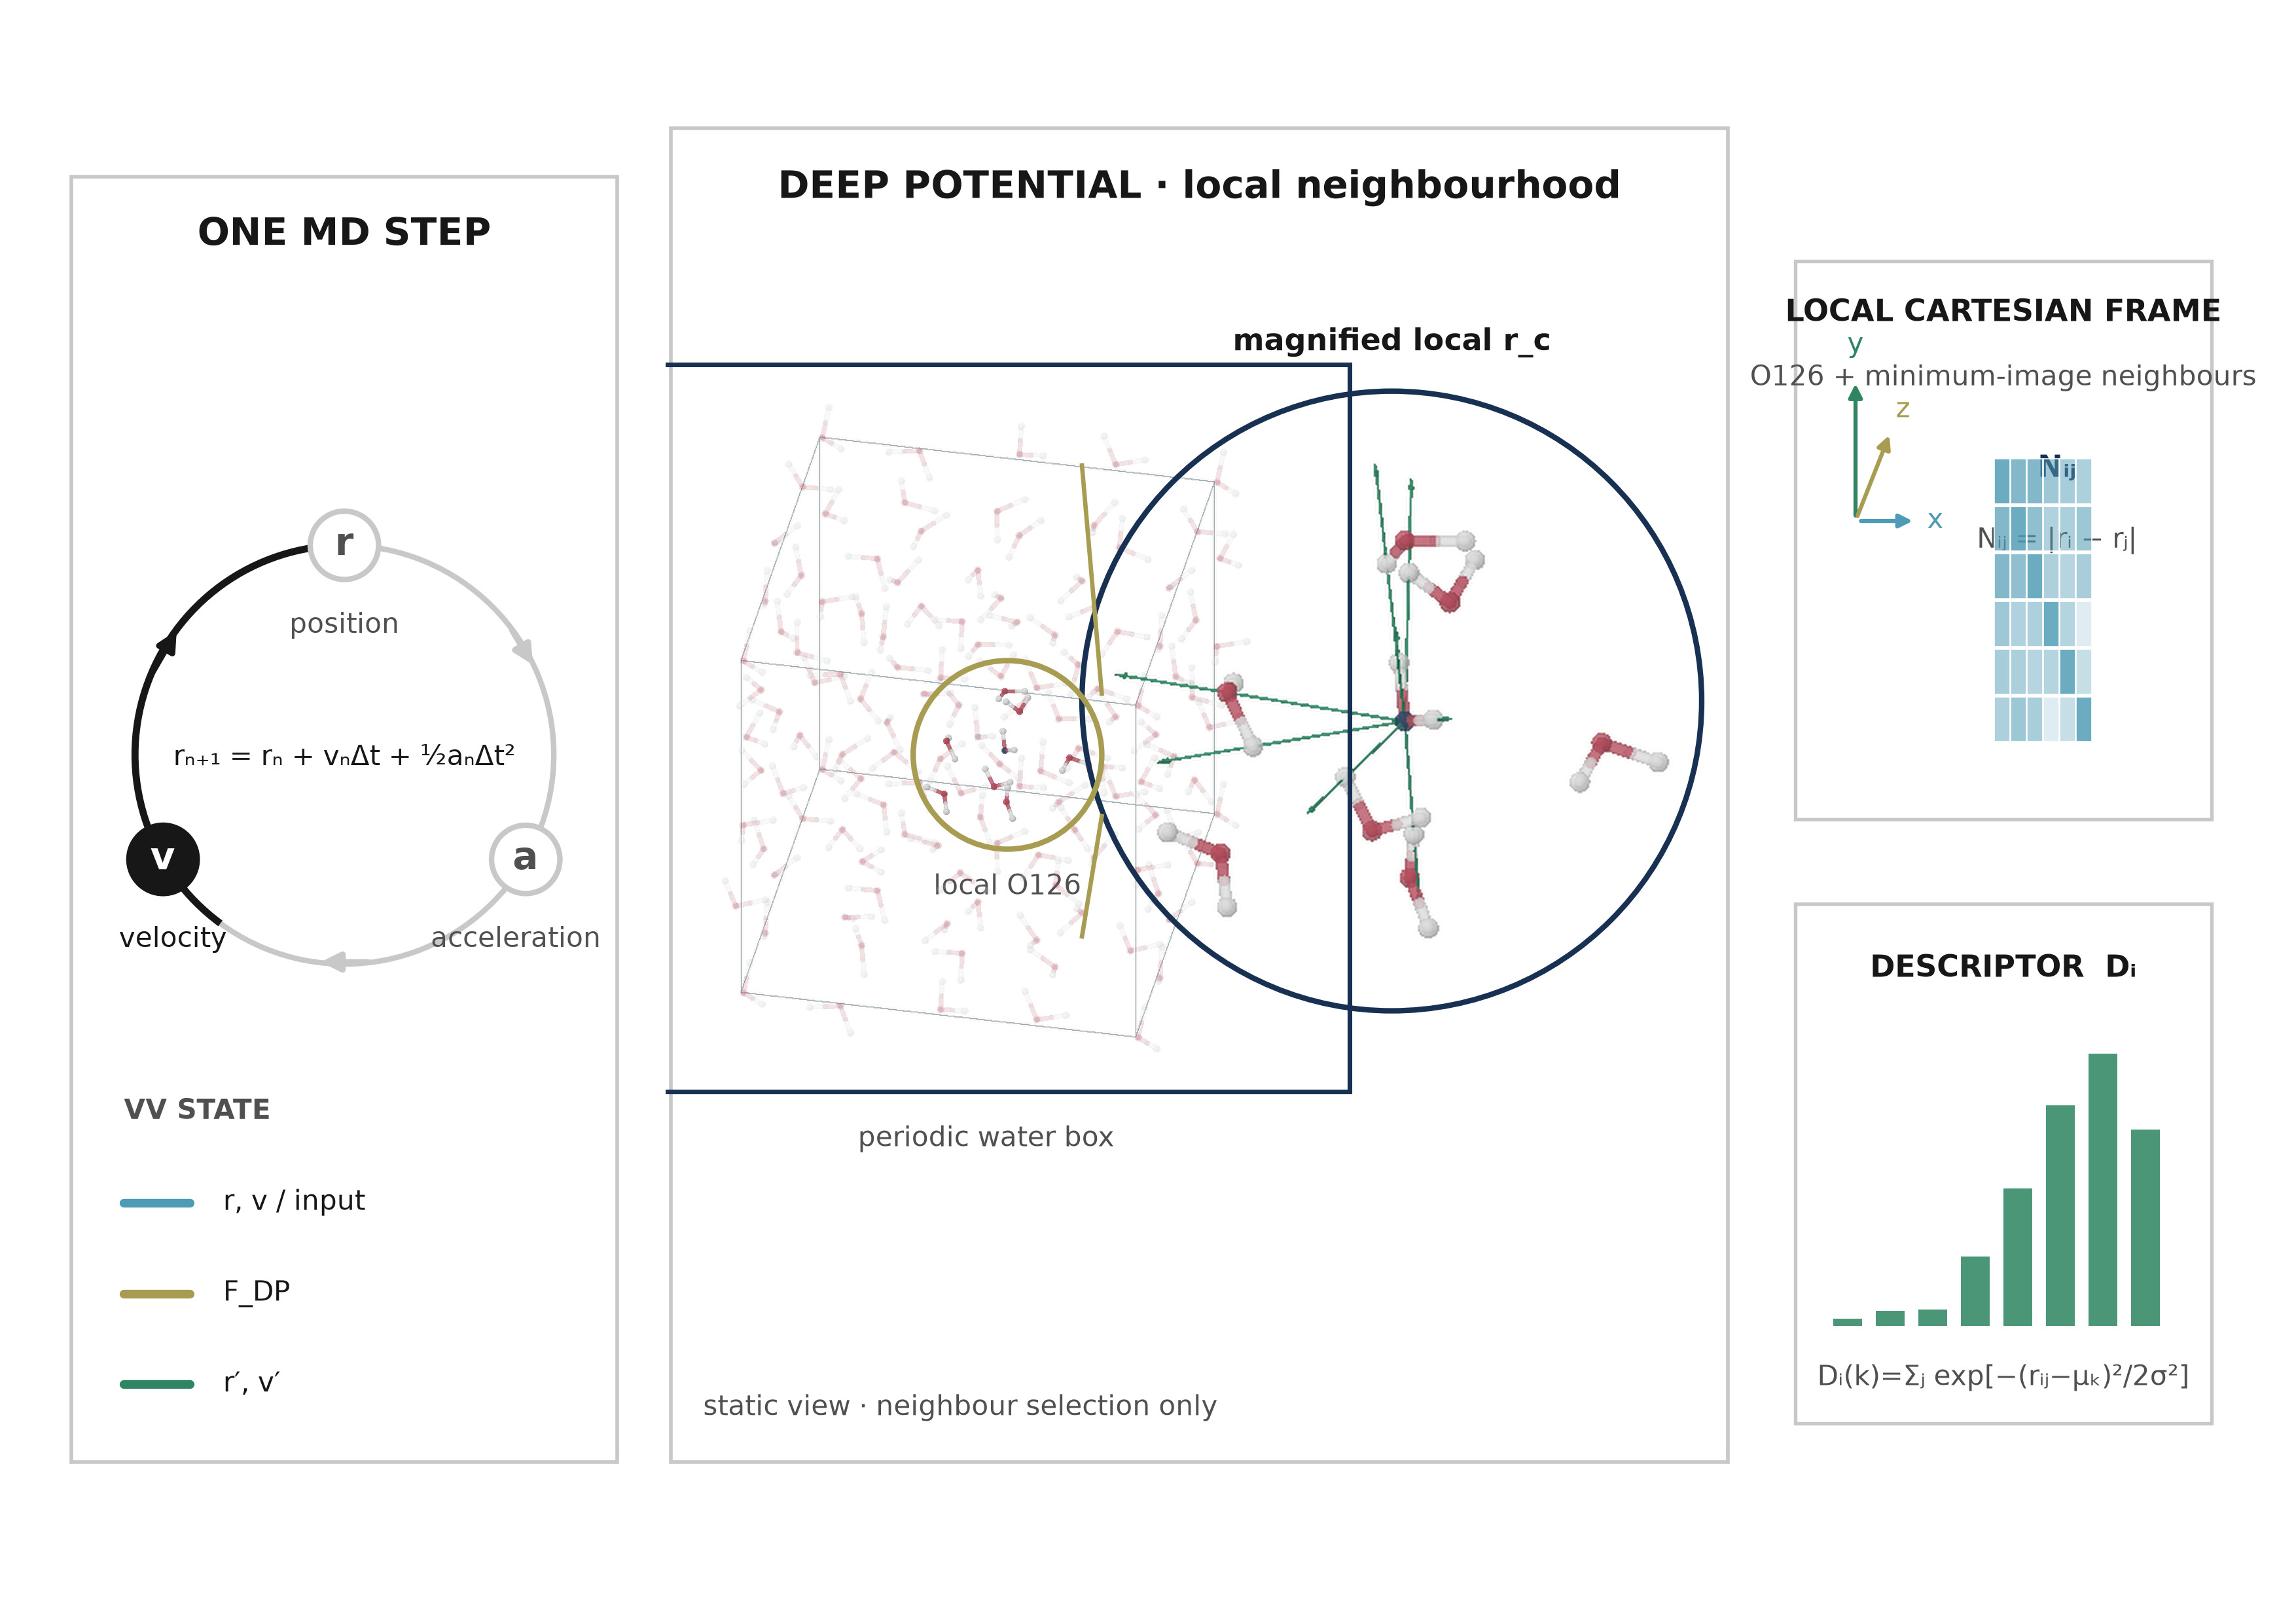
\includegraphics[width=0.93\textwidth]{../four_part_story/figures/04_deep_potential_md.png}
  \caption{Deep Potential MD 中从局域环境到原子力的映射。中心原子的截断邻域经过共享模型得到原子能，总能量的坐标梯度给出力，并返回外层积分器推进周期水盒。}
  \label{fig:dpmd}
\end{figure}

\subsection{机器学习势的表示边界}

现代 MLIP 很难用一条“后一代全面替代前一代”的序列概括。描述符、核方法、消息传递、等变表示、训练数据组织和部署效率在并行演化。表~\ref{tab:mlip}只给出定位，不把不同数据集上的误差横向硬比。

\begin{longtable}{>{\raggedright\arraybackslash}p{0.16\textwidth}>{\raggedright\arraybackslash}p{0.17\textwidth}>{\raggedright\arraybackslash}p{0.40\textwidth}>{\raggedright\arraybackslash}p{0.10\textwidth}}
\caption{代表性机器学习势的定位。论文与软件版本状态截至 2026 年 8 月。}\label{tab:mlip}\\
\toprule
方法 & 主要表示 & 对本文主线的意义 & 状态 \\
\midrule
\endfirsthead
\toprule
方法 & 主要表示 & 对本文主线的意义 & 状态 \\
\midrule
\endhead
BP-NNP & 对称函数+原子网络 & 确立高维势能面的局域原子能分解范式\cite{behler2007} & 已发表 \\
GAP/\allowbreak SOAP & 核回归+邻居密度 & 可系统改进的几何表示与高斯过程路线\cite{bartok2010} & 已发表 \\
Deep Potential & 局域环境+共享深网 & 能量、力、并行训练和大规模 MD 的统一实现\cite{han2018,zhang2018deepmd} & 已发表 \\
M3GNet & 材料图网络 & 面向多元素晶体的通用势与材料弛豫\cite{chen2022m3gnet} & 已发表 \\
CHGNet & 电荷知情图网络 & 把磁矩/电荷相关表征引入通用材料势\cite{deng2023chgnet} & 已发表 \\
MACE & 高体阶等变消息 & 以高阶等变消息提高表达效率\cite{batatia2022mace} & 已发表 \\
NEP & 神经演化势 & 强调较紧凑描述符和高效 CPU/GPU 推理\cite{fan2022nep} & 已发表 \\
eSEN & 平滑等变能量网络 & 强调势能面的高阶平滑性与物性预测\cite{fu2025esen} & 已发表/预印本版本 \\
DPA-2 & 多任务预训练 DP & 将 DP 推向跨数据集的大型原子模型\cite{zhang2024dpa2} & 预印本 \\
DPA-3 & 消息传递大型原子模型 & 统一描述符并扩展多任务/预训练部署\cite{deepmdkit2026dpa3} & 软件发布 \\
DPA-4 & SO(3) 等变消息模型 & 以精度--成本 Pareto 前沿为目标的新架构\cite{li2026dpa4} & 2026 预印本 \\
\bottomrule
\end{longtable}

模型名称之外，更值得检查四件事。第一，训练集是否覆盖目标温压、相态、缺陷和反应路径；第二，能量、力、virial 的损失权重是否支持目标观测量；第三，邻居截断和平滑函数是否足以描述目标非局域效应；第四，NVE 长期稳定性、声子、弹性、扩散和相变等下游量是否通过独立验证。测试集均方误差低，不等于轨迹永远稳定，也不等于自由能差可靠。

\section{采样问题：有限轨迹怎样支持统计结论}

\subsection{相关轨迹的有效样本数}

动力学轨迹通常同时承担两种任务：描述时间演化，或从某个系综估计统计量。二者的验证标准不同。平衡期（equilibration）用于消除初态记忆，生产期（production）才进入统计；但把前若干皮秒机械删除并不能证明已平衡。温度、能量、密度、结构序参量和目标观测量应从不同初态或不同轨迹比较其稳定性。

对时间序列 $A_t$，样本之间通常相关。若方差为 $\sigma_A^2$，积分自相关时间 $\tau_{\mathrm{int}}$ 决定有效样本数的量级：
\begin{equation}
  N_{\mathrm{eff}}\approx\frac{N\Delta t}{2\tau_{\mathrm{int}}}.
\end{equation}
保存一百万帧不代表有一百万份独立信息。分块平均把连续轨迹切成逐渐更长的块，观察块均值方差何时进入平台，可避免直接截断噪声很大的自相关函数\cite{flyvbjerg1989}. 报告平均值而不报告相关性、块长和误差条，往往比轨迹本身的数值误差更危险。

\subsection{系综控制的动力学时间尺度}

常规采样还要区分积分器与 thermostat/barostat。Velocity Verlet 解决确定性 Hamilton 部分；Langevin、Nos\'e--Hoover 链等改变动力学以采样目标温度；barostat 再引入体积或晶胞自由度。不同算法可能给出相同的平衡分布，却有不同的动力学时间尺度。若目标是扩散系数、粘度或时间关联函数，温控耦合强度不能只按“温度曲线最平”选择。

\subsection{自由能势垒的增强采样}

自由能势垒高于热涨落时，普通 MD 会在单个亚稳态中停留很久。增加总步数只有在能覆盖多次独立跃迁时才有效。增强采样通过偏置、约束或副本交换改变访问概率，再把偏置正确地重加权回目标分布。

伞形采样（umbrella sampling）在一组重叠窗口中给集体变量 $s(\bm R)$ 加谐和约束，分别采样后用 WHAM 或 MBAR 等方法拼接自由能\cite{torrie1977}. 它的优点是窗口可并行、覆盖范围明确；困难在于窗口布置、隐藏慢变量和相邻窗口重叠不足。

Metadynamics 沿集体变量轨迹不断沉积 Gaussian hills，逐渐填平已访问的自由能井，从而推动体系跨越势垒\cite{laio2002}. Well-tempered metadynamics 让 hill 高度随已积累偏置衰减，避免普通 metadynamics 无限制地填充；在适当条件下，偏置与自由能满足
\begin{equation}
  F(s)\simeq-\frac{\gamma}{\gamma-1}V(s,t)+C,
\end{equation}
其中 $\gamma=(T+\Delta T)/T$ 为 bias factor\cite{barducci2008}. 这个关系不是“动画跑久了自然成立”：集体变量必须区分慢模态，hill 宽度和沉积步长要解析局部扩散，重加权与收敛还需独立检查。

一维双阱能够直接区分普通 Langevin 动力学与 well-tempered metadynamics：无偏轨迹可能长期停留在单井，逐步沉积的偏置则增加跨垒事件，并可据此恢复无偏自由能。随机种子、时间步、摩擦、温度、hill 高度与宽度、沉积间隔、bias factor、跨阱次数和自由能均方误差共同规定这一数值实验的可复现条件。

\section{可信度问题：积分、模型与统计误差怎样区分}

一条 MD 轨迹至少叠加四类误差：
\begin{enumerate}
  \item \textbf{积分误差：} $\Delta t$、约束容差和离散算法造成；
  \item \textbf{势能面误差：} 经验势参数、电子结构近似或 MLIP 外推造成；
  \item \textbf{系综误差：} thermostat/barostat 与有限尺寸造成；
  \item \textbf{统计误差：} 有限轨迹、相关性和未跨越慢模态造成。
\end{enumerate}
这些误差不能用一个“能量曲线看起来稳定”替代。势函数错误时，积分器再好也只是在错误势能面上忠实运动；采样没收敛时，势函数再准也不能支持自由能结论；时间步过大时，温控器可能掩盖能量漂移，却同时改变动力学。

实践中可按以下顺序做收敛检查。先在小体系 NVE 上缩小时间步，检查总能量有界振荡、力连续性和目标结构量；再固定数值设置，比较势模型或电子结构层级；随后检查体系尺寸、截断、长程修正和系综参数；最后用独立轨迹、块平均和跨态次数估计统计误差。只有把这四层分开，才能知道“结果变了”究竟该改积分器、势函数还是采样策略。

\subsection{初态对目标观测量的约束}

开始计算前应先写清目标是平衡结构、热力学平均、输运系数、反应自由能，还是一段可解释的动力学。不同目标对轨迹长度、系综和输出频率的要求并不相同。若只关心径向分布函数，过密保存速度会增加 I/O 而没有收益；若要计算速度自相关和振动态密度，稀疏保存又会丢失高频信息。采样间隔因此应由目标观测量决定，而不是沿用软件默认值。

初始构型要先排除原子重叠、错误周期镜像和不合理键长。速度可从目标温度的 Maxwell--Boltzmann 分布抽样，但有限体系的一次随机实现不会自动具有零总动量；通常需要去除质心漂移，并在需要时去除整体转动。随后重新标定温度时，应使用扣除约束和整体运动后的实际自由度数。对含刚性水的体系，约束数目若被漏算，显示温度会产生系统偏差。随机种子、质量、单位制和自由度处理都应写入记录，否则“同一输入”仍可能无法复现。

\subsection{积分误差的时间步收敛}

不要直接在最昂贵的势函数上寻找合适步长。谐振子、单个水分子或小水簇已经足以暴露更新顺序、质量单位和速度半步错位。对 velocity Verlet，可分别保存式~\eqref{eq:vv-r}--\eqref{eq:vv-v}的中间状态，确认新力确实在新位置上计算，并检查下一步是否复用了 $\bm A_{n+1}$。再用一组逐次减半的 $\Delta t$ 测量坐标误差，二阶斜率比“看起来平滑”更有判别力\cite{swope1982,hairer2006}。

进入真实体系后，先跑短 NVE。合理现象是能量围绕一个窄区间振荡，缩小步长后振幅按预期下降；持续单向漂移则需要依次排查力不连续、邻居表更新、约束容差、SCF 未收敛和积分器实现。温度短时起伏在小体系中尤其常见；过强温控得到的一条过分平滑的温度线，反而可能掩盖真实动力学。只有 NVE 基线通过后，再引入 thermostat 或 barostat，调节耦合时间并验证目标系综。

\subsection{势能面误差的适用范围}

每一种势函数都应先脱离 MD 循环单独测试。对解析势，在随机但物理合理的构型上比较解析力和中心有限差分；对 AIMD，改变 SCF 阈值、积分网格和基组，观察力而不只是总能量是否收敛；对 MLIP，核对自动微分力、virial、元素映射和单位制，并专门扫描截断半径附近的连续性。能量误差可以被一个常数平移掩盖，力和二阶导数却直接控制轨迹、声子和稳定性。

MLIP 还需要外推诊断。一个模型在随机测试集上误差很低，可能只是因为训练集和测试集来自同一条相邻轨迹。更严格的划分应按构型来源、温压区间、相态或化学组成分组；生产轨迹中则监测模型委员会偏差、描述符距离或其他适用域指标。发现异常构型后，先用电子结构重新标注并检查是否具有物理意义，再决定是否加入训练集。把数值爆炸后的非物理重叠直接当成普通训练样本，会让数据量增加，却未必改善目标区域。

\subsection{模型体系的解释尺度}

水二聚体不是液态水的缩小版，它的价值在于可解释。六个原子的构型足以清楚展示 O--O 距离、氢键取向、LJ 分量、电子密度变化和核力方向；SCF 的每一次更新也能在固定分子平面上稳定呈现。因而它适合解释“某一步为什么得到这支力”，却不适合证明体相密度、扩散或氢键网络已经收敛。

六十四水盒恰好补上统计和周期环境。选定一个中心原子后，$6$~\AA{} 球内邻居来自真实周期最小镜像，局域环境足以说明 Deep Potential 如何把大量原子压缩成可并行的邻域计算；完整轨迹又能用于径向分布和扩散等体相量。相应代价是画面更拥挤，单个力分量不再直观。因此，二聚体负责可解释的因果链，水盒负责展示可扩展性和真实局域环境；二者不能互相替代，也不应在同一张图里争夺视觉中心。

\subsection{统计误差的自由能收敛}

一条轨迹是否够长，不能由纳秒或帧数单独判断。先用多个时间起点计算 running average，再比较不同初态的独立副本；对慢变量，检查每条轨迹是否多次往返于相关亚稳态。随后以逐步增加的块长做分块平均，直到标准误差进入平台\cite{flyvbjerg1989}. 若平台始终没有出现，应报告“当前轨迹不足以估计误差”，而不是选择一个看起来合适的块长。

增强采样同样需要独立验证。Well-tempered metadynamics 中，自由能曲线暂时不再变化可能只是集体变量空间的一部分被填平。更可靠的证据包括多次可逆跨垒、不同时间窗口重建结果一致、独立重复的自由能差相符，以及重加权后未偏置自由度的分布稳定。若隐藏慢变量没有被选入 CV，继续沉积 hills 可能改变表面形状，却不真正增加独立采样。

最后应保存一份能够重建结论而不只重播动画的最小档案：初始结构、势模型哈希、软件版本、随机种子、时间步、系综参数、约束、截断和长程设置、SCF 阈值、平衡期判据、生产期范围以及分析脚本。轨迹文件很大时可以降低保存频率或保存关键统计量，但元数据不能省略。这些元数据是区分物理变化与软件变化的实验条件，而非附加文档。

\section{从初态到统计结论的闭合关系}

从斜抛运动到六十四个水分子的 Deep Potential 轨迹，数学形式始终没有离开初值问题。变化的是力的来源、每步成本和可访问的时间尺度。显式 Euler 说明局部看似合理的更新会怎样破坏长期结构；velocity Verlet 通过对称、辛的分裂，在一次新力计算的成本下给出可靠的二阶推进；经验势把电子响应压缩进手写函数，AIMD 在每个离子步嵌入真实 SCF，机器学习势则试图把高成本势能面蒸馏成可扩展的局域模型。

分子动力学的完整计算链由势能面、积分器、系综和统计分析共同组成：物理模型定义原子受力，积分器推进离散轨迹，系综方法规定目标分布，相关性分析判断有限轨迹包含多少独立信息。本文的水分子、水二聚体和水盒案例把抽象更新、真实结构、电子迭代与统计收敛置于同一条可核查的因果链中。


\section*{参考文献}
\vspace{-7pt}
\begin{multicols}{2}
\raggedright
\raggedcolumns
\setlength{\columnsep}{10pt}
\fontsize{9}{10.5}\selectfont
\printbibliography[heading=none]
\end{multicols}

\end{document}
